\chapter{Local observables and regular current actions}
\label{chap:current-actions-local-observables}

A detector occupies an open region, whereas a Taylor coefficient is
attached to a point. The free field construction must accommodate both.
Smearing a field with a smooth compactly supported function gives the
first kind of measurement. The residue pairing of
Chapter~\ref{chap:two-dimensional-free-fields} gives the second.
Products of smeared fields require functions of several positions.
Their symmetry operators require control of infinitely many Taylor modes.

The two constructions admit explicit formulas. Smooth kernels give
complexes of observables with multiplication on disjoint regions.
A finite-configuration covering condition reconstructs these complexes
from smaller regions, including all powers of $\hbar$.
Polynomial matrix currents act on the free modes by locally finite
quadratic operators. Their commutators realize the polynomial current
Lie algebra exactly. Comparing these operators with singular current
insertions requires an additional map, whose domain matters.

\section{Measurements with several positions}
\label{sec:clo-smooth-kernels}

Let $M$ be either $\mathbb C^2$ or
$\mathbb R^2\times\mathbb C^2$, with the coordinates and orientations
of Chapter~\ref{chap:two-dimensional-free-fields}.
In the mixed case every coefficient is jointly smooth in
$t,s,z_1,z_2,\bar z_1,\bar z_2$.
The finite exterior algebra of mixed forms is part of the field bundle.
It imposes no separation of the coordinate dependence.

Write $E$ for the finite-rank graded complex vector bundle of fields.
For the holomorphic theory its sections are the pair $(\gamma,\beta)$.
For the mixed theory they are $(\alpha,\beta)$.
Their differential $Q_E$ has degree one and is the differential already
specified in that chapter. The coefficient degrees occupy a finite interval.
Write
\[
 E^!=E^\vee\otimes\operatorname{Dens}_M,
 \qquad (E^\vee)^j=(E^{-j})^\vee.
\]
Here $\operatorname{Dens}_M$ is the complexified density line.
The fixed orientation identifies its sections with top forms for integration.

A compactly supported section $f$ of $E^!$ gives a linear observable
\[
 \ell_f(\phi)=\int_M\langle f(x),\phi(x)\rangle,
 \qquad \phi\in\Gamma^\infty(M,E).
\]
The support of $f$ specifies the detector region.
The field $\phi$ need not have compact support.
For homogeneous graded fields, evaluation uses the Koszul rule:
exchanging degrees $a,b$ gives $(-1)^{ab}$.
The degree of $\ell_f$ is the degree of its dual coefficient $f$.

Two detectors can have a correlated response. For scalar even components,
such a measurement has the form
\[
 F_K(\phi)=\int_{U\times U}K(x,y)\phi(x)\phi(y),
 \qquad K\in\Gamma_c^\infty(U^2,\operatorname{Dens}_M^{\boxtimes2}).
\]
The symbol $\boxtimes$ means that each factor is pulled back from its
own position and the resulting bundles are tensored together.
Even when both positions lie in one coordinate box, $K$ need not be a
finite sum $\sum_a f_a(x)g_a(y)$.
For example, choose bump functions $\chi,\psi$ that equal one on
intervals and consider $\chi(u)\psi(v)e^{uv}$.
If it were a finite sum of separated functions, all functions
$u\mapsto e^{uv}$ on the smaller interval would lie in one
finite-dimensional vector space. For any distinct $v_1,\ldots,v_N$,
their linear independence follows by differentiating at one point:
the resulting Vandermonde determinant is nonzero.
There is no uniform finite bound on $N$.

This measurement fixes the kernel space to be used. For $n\geq1$, put
\begin{equation}\label{eq:clo-kernel-space}
 \mathscr O_n(U)=
 \Gamma_c^\infty\bigl(U^n,(E^!)^{\boxtimes n}\bigr)_{S_n},
 \qquad
 \mathscr O_{\mathrm{poly}}(U)=\bigoplus_{n\geq0}\mathscr O_n(U).
\end{equation}
The subscript identifies a kernel with its permutations, including the
Koszul signs of its coefficient factors. Thus it denotes coinvariants.
Over $\mathbb C$, averaging over the finite group identifies coinvariants
with invariant kernels. Put $\mathscr O_0(U)=\mathbb C$ for every $U$,
including $U=\varnothing$. Its element $1$ is the constant measurement.
For $n>0$, $\mathscr O_n(\varnothing)=0$.

The integer $n$ is polynomial degree, also called particle number here.
It is distinct from cohomological degree, which is the sum of the
coefficient degrees. A polynomial observable has a finite sum of
particle numbers. Its degree-$n$ kernel can nevertheless be an arbitrary
jointly smooth compactly supported function of its $n$ positions.
Evaluation integrates that kernel against $\phi^{\otimes n}$.
There is no $1/n!$ in this convention.
Consequently multiplication concatenates slots before passing to
coinvariants.

For a fixed compact subset $K\subset U^n$, the smooth topology is
given by suprema of all derivatives on $K$.
Allowing $K$ to vary gives the compact-support inductive limit topology.
For linear maps, continuity on all fixed-support spaces gives continuity
on this inductive limit. Bilinear multiplication requires the separate
estimates of Section~\ref{sec:clo-support-estimates}.
Cohomology will mean algebraic kernels modulo algebraic images.
No closed-image assertion is implicit.

\section{The free differential on measurement kernels}
\label{sec:clo-free-differential}

The equations of motion act on a linear measurement by the graded
transpose of $Q_E$:
\[
 \ell_{Q_{\mathrm{obs}}f}(\phi)
 =-(-1)^{|f|}\ell_f(Q_E\phi).
\]
Integration by parts defines the compactly supported smooth coefficient
$Q_{\mathrm{obs}}f$. There is no boundary contribution.
On $n$ slots the differential is the tensor differential, with sign
$(-1)^{|f_1|+\cdots+|f_{i-1}|}$ in slot $i$.
This also defines it on a general joint kernel by differential operators
in the separate position variables. It preserves particle number and
squares to zero.

The second operation measures a contraction at coincident positions.
The odd field pairing is fiberwise nondegenerate and density-valued.
Its inverse gives a contraction of two dual-density coefficients to one
density, of degree one. Fix its sign by requiring
\[
 \Delta(x\xi)=1
\]
for a conjugate pair of linear coordinates with $x$ even,
$\xi$ odd, and $|x|+|\xi|=-1$.
This is the convention of Section~\ref{sec:gaussian-bv-algebra}.
Write $\mathsf k(f,g)$ for the integral of this coefficient contraction
after setting the two positions equal. Thus $\mathsf k$ is a scalar
pairing of degree one on compactly supported linear kernels.
It is graded symmetric:
\[
 \mathsf k(f,g)=(-1)^{|f||g|}\mathsf k(g,f).
\]
The pairing can be nonzero only when $|f|+|g|=-1$.

Define $\Delta:\mathscr O_n(U)\to\mathscr O_{n-2}(U)$ by summing
over unordered pairs of slots. Each summand restricts the two selected
positions to their diagonal, contracts their coefficients, and integrates
that position. The remaining positions retain their order.
On a product of homogeneous linear measurements this reads
\begin{equation}\label{eq:clo-contraction-sign}
 \Delta(f_1\cdots f_n)=
 \sum_{i<j}(-1)^{\epsilon_{ij}}\mathsf k(f_i,f_j)
 f_1\cdots\widehat f_i\cdots\widehat f_j\cdots f_n,
\end{equation}
where
\[
 \epsilon_{ij}=
 |f_i|\sum_{k<i}|f_k|
 +|f_j|\sum_{\substack{k<j\\k\ne i}}|f_k|.
\]
The exponent moves the selected pair to the first two slots.
Formula~\eqref{eq:clo-contraction-sign} determines the coefficient
permutations for a general joint kernel as well.

Smoothness permits the diagonal restriction.
Compact support permits integration and leaves compact support in the
remaining variables. Differentiation in those variables passes under the
integral, proving smoothness of the result.
For a compact input support, every output derivative is bounded by
finitely many input derivative seminorms times a finite integration volume.
This also proves continuity.

\begin{proposition}\label{prop:clo-bv-identities}
For both free field bundles,
\[
 Q_{\mathrm{obs}}^2=0,\qquad \Delta^2=0,\qquad
 Q_{\mathrm{obs}}\Delta+\Delta Q_{\mathrm{obs}}=0.
\]
The operator $\Delta$ has degree one and lowers particle number by two.
\end{proposition}

\begin{proof}
The first identity is the dual of $Q_E^2=0$.
For the second, two contractions can use only disjoint pairs of slots.
The two possible orders contract the same four positions and integrate
the same compactly supported smooth kernel.
Each contraction has odd degree. Exchanging their order changes the
Koszul sign by minus one, so the two terms cancel.

Invariance of the field pairing under $Q_E$, followed by compact-support
integration by parts, gives
\[
 \mathsf k(Q_{\mathrm{obs}}f,g)
 +(-1)^{|f|}\mathsf k(f,Q_{\mathrm{obs}}g)=0.
\]
Apply $Q_{\mathrm{obs}}$ to~\eqref{eq:clo-contraction-sign}.
Terms in uncontracted slots cancel against the same terms in
$\Delta Q_{\mathrm{obs}}$, since the contraction has degree one.
The displayed compatibility cancels the terms in the contracted pair.

These calculations apply to separated kernels. They also apply to joint
kernels by continuity. For completeness, separated smooth kernels are
dense after allowing a fixed slightly larger compact support.
Cover the input support by finitely many product coordinate boxes and
use a smooth partition of unity on that finite cover.
For each resulting kernel, take its smooth periodic extension from a
larger box, where it is zero near the boundary.
Its Fourier series converges with every derivative.
Each Fourier term separates the position variables.
Multiplying by a product of bump functions that equals one on the
support keeps all approximants in one fixed compact subset.
The same construction applies to each of the finitely many coefficient
components. Continuity therefore extends all three identities.
\end{proof}

A single even coordinate and its odd conjugate already show the
quantum correction. If their smeared linear kernels are $f$ and $g$,
then
\[
 \Delta(\ell_f\ell_g)=\mathsf k(f,g).
\]
In the scalar Darboux normalization, with coefficient functions
$u,v$ relative to the fixed volume density, this is $\int_M uv\,dV$.
It vanishes for disjoint supports. An overlap can produce a nonzero
constant measurement.

Let $\hbar$ have cohomological degree zero. Define
\begin{equation}\label{eq:clo-quantum-differential}
 d=Q_{\mathrm{obs}}+\hbar\Delta,
 \qquad
 d^2=0.
\end{equation}
The Batalin--Vilkovisky bracket is the degree-one operation
\[
 \{F,G\}=(-1)^{|F|}
 \bigl(\Delta(FG)-(\Delta F)G-(-1)^{|F|}F\Delta G\bigr).
\]
It sums contractions with one slot in each factor.
Thus
\[
 d(FG)-(dF)G-(-1)^{|F|}F(dG)
 =\hbar(-1)^{|F|}\{F,G\}.
\]
The Gaussian calculation becomes a statement about overlap of detector
regions. Products on disjoint regions will be chain maps.

\section{Smooth estimates and support bounds}
\label{sec:clo-support-estimates}

Combining two detector responses multiplies their kernels in separate
positions. The derivative estimate has to retain both supports.
Use the global real coordinates on $M$, the fixed volume density, and
a homogeneous coefficient basis for $E^!$.
For a compact subset $K\subset U^n$, let $\mathscr D_K$ be the space
of smooth coefficient kernels supported in $K$, before permutation
identifications. For $m\geq0$, put
\[
 \|f\|_{K,m}=
 \max_{|\alpha|\leq m}\sup_{x\in K}|\partial^\alpha f(x)|.
\]
The coefficient norm is the maximum of the absolute values of the
finitely many coefficient entries. The multi-index $\alpha$ differentiates
all real position coordinates. These seminorms define the fixed-support
Fr\'echet topology.
For $K=\varnothing$ the seminorm is zero.

For compact $K\subset U^p$ and $L\subset V^q$, external multiplication
is the bilinear map
\[
 \mathscr D_K\times\mathscr D_L\longrightarrow\mathscr D_{K\times L},
 \qquad (f,g)\longmapsto f\boxtimes g.
\]
Derivatives in the first group act only on $f$, and derivatives in the
second group act only on $g$. Hence
\begin{equation}\label{eq:clo-fixed-support-estimate}
 \|f\boxtimes g\|_{K\times L,m}
 \leq\|f\|_{K,m}\|g\|_{L,m}.
\end{equation}
In particular, this map is jointly continuous for fixed $K,L$.
After extension and averaging over $S_{p+q}$, the support lies in
$\bigcup_{\sigma\in S_{p+q}}\sigma(K\times L)$.
Each permutation preserves the maximum derivative seminorm.
The normalized average therefore satisfies the same estimate.
This proves fixed-support bilinear continuity for multiplication of
coinvariant kernels as well.

To allow supports to vary without losing the estimate, specify which
families of measurements are bounded. A subset $B\subset\mathscr O_n(U)$
is called \emph{bounded} if its invariant representatives have a common
compact support $K\subset U^n$ and
\[
 \sup_{f\in B}\|f\|_{K,m}<\infty\qquad\text{for every }m\geq0.
\]
The invariant representative is the normalized permutation average of
any representative. It is unique, and its support can be taken invariant
under $S_n$. For $n=0$ use ordinary bounded subsets of $\mathbb C$.
This definition fixes the boundedness structure used here.
For a finite-rank joint-kernel space, use the same definition before
or after its stated within-group permutation average.
A multilinear map is called bounded if it sends a product of bounded
subsets into a bounded subset.
Direct sums carry the locally convex direct-sum topology.
A subset of such a sum is called bounded when one finite set of
summands contains it and every projection is bounded in the stated sense.
Thus bounded families in $\mathscr O_{\mathrm{poly}}^q(U)$ have a
common finite particle bound and smoothly bounded kernels at each
particle number. All these definitions are made in a fixed cohomological
degree $q$.
These families contain all singletons and are closed under subsets and
finite unions. Sums and scalar multiples with bounded scalar coefficients
remain bounded, since their supports have a finite compact union and
their derivative bounds add.

\begin{proposition}\label{prop:clo-bounded-multiplication}
External multiplication and the symmetrized multiplication of smooth
compact kernels are bounded. Extension, the free differential, the
diagonal contraction, and permutation averaging are continuous linear
maps on their stated compact-support spaces and preserve bounded sets.
\end{proposition}

\begin{proof}
For bounded input families, choose their common supports $K,L$.
Equation~\eqref{eq:clo-fixed-support-estimate} gives a common output
support and a uniform bound on every output derivative.
Extension preserves derivatives on the support.
Permutation averaging has only finitely many terms.
The free differential differentiates at most once, with fixed coefficient
maps, so each output seminorm is bounded by a constant times the input
seminorm of order $m+1$.

For a diagonal contraction, the output support lies in the compact
projection of the input support intersected with the selected diagonal.
Choose a compact integration box containing the selected position
projection. Differentiation in the remaining variables commutes with
integration. The output seminorm of order $m$ is at most the box volume
times the coefficient-contraction norm times the input seminorm of
order $m$. The sum over pairs is finite at each particle number.
These estimates prove preservation of bounded sets and continuity on
every fixed-support space. For these linear maps, the defining
inductive-limit property then gives continuity on the full
compact-support spaces.
\end{proof}

Joint continuity of a bilinear map does not follow from the same
inductive-limit argument. A counterexample occurs in a degree-zero
scalar component of the holomorphic theory.
Identify $M$ with $\mathbb R^4$, and put
$a_n=(n,0,0,0)$ for $n\geq1$.
On smooth compact two-position kernels define the seminorm
\[
 p(F)=\sup_{n\geq1}
       |\partial_{x_1}^{n}F(0,a_n)|.
\]
For every compact support $H\subset M^2$, only finitely many points
$(0,a_n)$ belong to $H$. All other evaluations vanish on
$\mathscr D_H$. Thus the restriction of $p$ to $\mathscr D_H$ is a
finite maximum of continuous derivative evaluations.
By the definition of the locally convex inductive-limit topology, $p$
is continuous on the full compact-support space.
Its restriction to symmetric kernels is continuous as well.

Take disjoint opens
\[
 U_0=B(0,1/4),\qquad U_1=\bigcup_{n\geq1}B(a_n,1/4).
\]
Here $B(a,r)$ denotes the Euclidean open ball with center $a$ and radius $r$.
Suppose the symmetric external product from
$\Gamma_c^\infty(U_0)\times\Gamma_c^\infty(U_1)$ were jointly
continuous into $\mathscr O_2(M)$ in these topologies.
There would be zero neighborhoods $V,W$ such that
$p(f\boxtimes_{\mathrm{sym}}g)\leq1$ for $f\in V,g\in W$.
Here
\[
 (f\boxtimes_{\mathrm{sym}}g)(x,y)
 =\tfrac12\bigl(f(x)g(y)+f(y)g(x)\bigr).
\]
Choose a compact neighborhood $K$ of zero inside $U_0$ and a smooth
bump $\chi$ supported there, with $\chi=1$ near zero.
The neighborhood $V\cap\mathscr D_K$ contains
$\{f:\|f\|_{K,m}<\epsilon\}$ for some $m$ and $\epsilon>0$.
For sufficiently small fixed $c>0$, every function
\[
 f_T(x)=cT^{-m}\chi(x)e^{iTx_1},\qquad T\geq1,
\]
belongs to that neighborhood. Indeed, the product rule bounds all
derivatives through order $m$ by a constant times $c$, uniformly in $T$.
Choose an integer $n>m$.
Since $W$ absorbs scalar multiples of any fixed test function, it contains
a function $g$ supported near $a_n$ with $g(a_n)=\lambda\ne0$.
Its support is disjoint from $K$.
The chosen derivative of the symmetric product is
\[
 \partial_{x_1}^{n}
 (f_T\boxtimes_{\mathrm{sym}}g)(0,a_n)
 =\tfrac12 c\lambda i^nT^{n-m}.
\]
The other symmetric term vanishes because $g$ is zero near zero.
The displayed quantity is unbounded as $T\to\infty$, a contradiction.

Thus disjoint multiplication is bounded and jointly continuous on fixed
supports, while its bilinear map on the full LF spaces is not jointly
continuous. Here LF denotes the locally convex inductive limit of the
fixed-support Fr\'echet spaces along a compact exhaustion.
The continuous linear structural maps below instead start with actual
joint-kernel spaces. No tensor-product universal property is needed to
construct those maps.

\section{Two completions and the series they permit}
\label{sec:clo-completions}

Perturbation theory allows more field insertions at higher powers of
$\hbar$. Fix $m\geq1$ and put
\[
 R_m=\mathbb C[\hbar]/(\hbar^m),\qquad
 \mathscr O_m(U)=
 (\mathscr O_{\mathrm{poly}}(U)\otimes R_m,d).
\]
Reduction of coefficients gives surjective chain maps
$\mathscr O_{m+1}(U)\to\mathscr O_m(U)$.
Define
\begin{equation}\label{eq:clo-hbar-completion}
 \widehat{\mathscr O}(U)=\varprojlim_m\mathscr O_m(U)
 =\mathscr O_{\mathrm{poly}}(U)[[\hbar]].
\end{equation}
The equality describes the underlying graded vector space.
Limits and products of complexes are taken in each cohomological degree.
An arbitrary element of the underlying graded space is a finite sum
of homogeneous elements.
In degree $q$, an element is $\sum_{r\geq0}\hbar^r F_r$, with
$F_r\in\mathscr O_{\mathrm{poly}}^q(U)$ for every $r$.
Every coefficient is a finite polynomial in particle number.
Its differential has coefficient
$Q_{\mathrm{obs}}F_r+\Delta F_{r-1}$, where $F_{-1}=0$.
Multiplication uses the finite sum $\sum_{a+b=r}F_aG_b$ at order $r$.
The topology is the inverse limit topology, together with the smooth
kernel topology in each finite quotient.

For a nonzero linear observable $x$ of cohomological degree zero, the series
\[
 \sum_{r\geq0}\hbar^r x^{2r}
\]
is allowed. Its polynomial degrees have no common bound.
In contrast, $\sum_{n\geq0}x^n$ at order $\hbar^0$ is excluded.
The increasing polynomial-degree filtration is exhaustive on
$\mathscr O_m$, but not on $\widehat{\mathscr O}$.
This distinction affects descent.

A formal function of arbitrarily many particle numbers requires another
completion. The free contraction supplies a compatible weight:
\[
 w=n+2r\quad\text{on}\quad \hbar^r\mathscr O_n(U).
\]
Both terms of $d$ preserve $w$.
Write
\[
 \mathscr O^{(w)}(U)=
 \bigoplus_{\substack{n,r\geq0\\n+2r=w}}
       \hbar^r\mathscr O_n(U),
 \qquad
 \mathscr O^{\mathrm{wt}}(U)=\prod_{w\geq0}\mathscr O^{(w)}(U).
\]
Every fixed-weight sum is finite. Multiplication adds weights, so each
output weight receives finitely many input weights.
The product topology makes the linear differential $d$ continuous.
At $\hbar=0$, the degree-$q$ part of this completion is
$\prod_n\mathscr O_n^q(U)$.
It permits $\sum_n x^n$ as a formal observable, with no claim of
convergence on numerical fields.

There is an injective map commuting with multiplication and differential,
$\widehat{\mathscr O}(U)\to\mathscr O^{\mathrm{wt}}(U)$.
It rearranges the coefficients indexed by $(n,r)$ along their weights.
Its image consists of the arrays with only finitely many nonzero
particle numbers at each fixed $r$.
The two completions therefore retain different observables.
Quotienting only by high particle number would not define a quantum
complex: $\hbar\Delta$ can send particle number $N$ to $N-2$.
Weight truncation avoids that defect.

Boundedness in the completions is also specified coefficientwise.
A subset of $\widehat{\mathscr O}^{q}(U)$ is bounded when its
coefficient of each $\hbar^r$ is a bounded subset of
$\mathscr O_{\mathrm{poly}}^{q}(U)$.
Its particle bound and compact supports may depend on $r$.
A subset of $(\mathscr O^{\mathrm{wt}})^q(U)$ is bounded when its
projection to each weight is bounded in that finite direct sum.
Equivalently, each $(n,r)$ coefficient has a common compact support
and uniform bounds on all derivatives, with no uniform restriction
across different $(n,r)$.

These definitions make multiplication bounded in both completions.
At fixed $\hbar$ order $r$, the output uses only the finitely many
pairs of coefficient orders $a+b=r$.
Bounded input families have finite particle bounds at each such order.
Thus the output has a finite particle bound, a finite union of compact
supports, and derivative bounds obtained by summing
\eqref{eq:clo-fixed-support-estimate} finitely many times.
At fixed weight, both the weight decompositions and their particle
decompositions are finite, and the same argument applies.
The estimates for $Q_{\mathrm{obs}}$ and $\Delta$ prove that $d$
preserves bounded sets and is continuous and linear on both completions.
There is no joint-continuity assertion for their multiplication in the
displayed topologies. Restricting to linear kernels at order zero and
projecting to the two-particle coefficient at order zero recovers the
preceding counterexample.

\section{Multiplication in disjoint regions}
\label{sec:clo-disjoint-products}

Let $U_1,\ldots,U_k$ be pairwise disjoint open subsets of $U$.
To combine detectors, the input must include joint smooth kernels on
all their position variables. Define the tensor used for this purpose by
\begin{equation}\label{eq:clo-kernel-tensor}
 \widehat{\bigotimes}_{i=1}^k{}^{\!\mathrm{ker}}
     \widehat{\mathscr O}(U_i)
 :=\varprojlim_m
 \left[
 \bigoplus_{n_1,\ldots,n_k\geq0}
 \Gamma_c^\infty\left(
   \prod_iU_i^{n_i},
   \boxtimes_i(E^!)^{\boxtimes n_i}\right)_{\prod_iS_{n_i}}
 \otimes R_m\right].
\end{equation}
The notation names exactly the displayed space.
Each finite quotient carries the locally convex direct-sum topology of
the displayed joint-kernel spaces, with their compact-support topologies.
The completed domain carries the inverse-limit topology.
Its bounded subsets have bounded projections in every finite quotient,
using the joint-kernel and direct-sum definitions above.
Its differential acts in all slots and contracts only within each group.
It requires no identification with an unspecified topological tensor
product. The algebraic tensor of separated measurements maps into it by
external multiplication of kernels.

Extend the kernel by zero to $U^{n_1+\cdots+n_k}$ and pass from
within-group permutations to all permutations. This gives
\begin{equation}\label{eq:clo-factorization-product}
 \mu_{U_1,\ldots,U_k;U}:
 \widehat{\bigotimes}_{i=1}^k{}^{\!\mathrm{ker}}
 \widehat{\mathscr O}(U_i)\longrightarrow\widehat{\mathscr O}(U).
\end{equation}
Extension by zero is smooth because the input support is compact inside
its open domain. It commutes with the differential operator
$Q_{\mathrm{obs}}$.
Any contraction joining two different groups restricts to the empty
diagonal: one point cannot belong to two disjoint $U_i$.
Thus every such contraction vanishes, and $\mu$ is a chain map.
It is continuous and linear on the displayed joint-kernel domain:
on each fixed support it is a finite permutation average after extension.
Continuity passes to its direct sums and then to the inverse limit.
The same support and derivative estimates show that it preserves bounded
sets. Its induced multilinear operation on separate observable spaces
is bounded, with fixed-support continuity as proved above.

Nested products agree. For example, if $U_1,U_2\subset V_1$,
$U_3\subset V_2$, and $V_1,V_2\subset U$ are disjoint, then
\[
 \mu_{V_1,V_2;U}\bigl(\mu_{U_1,U_2;V_1}(F_1,F_2),F_3\bigr)
 =\mu_{U_1,U_2,U_3;U}(F_1,F_2,F_3).
\]
Both sides extend the same kernel and make the same final permutation
identifications. Reordering opens has precisely the Koszul sign.
The empty list gives the unit map $\mathbb C[[\hbar]]\to
\widehat{\mathscr O}(U)$.
One open gives its extension map.
These operations, with their nesting and permutation identities, are
the structure called a prefactorization algebra in this explicit
smooth-kernel setting.

\begin{figure}[htbp]
\centering
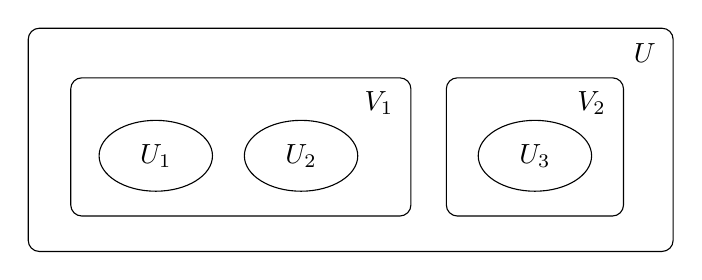
\begin{tikzpicture}[scale=.9]
 \draw[rounded corners] (-.6,-1.35) rectangle (8.5,1.8);
 \node at (8.1,1.45) {$U$};
 \draw[rounded corners] (0,-.85) rectangle (4.8,1.1);
 \node at (4.35,.75) {$V_1$};
 \draw[rounded corners] (5.3,-.85) rectangle (7.8,1.1);
 \node at (7.35,.75) {$V_2$};
 \draw (1.2,0) ellipse (.8 and .5);
 \draw (3.25,0) ellipse (.8 and .5);
 \draw (6.55,0) ellipse (.8 and .5);
 \node at (1.2,0) {$U_1$};
 \node at (3.25,0) {$U_2$};
 \node at (6.55,0) {$U_3$};
\end{tikzpicture}
\caption{Combining the first two detector regions before adjoining the
third gives the same extended kernel as the direct three-region product.
Disjointness removes every contraction between the outer groups.}
\label{fig:clo-nesting}
\end{figure}

For a disjoint union $U=U_1\sqcup\cdots\sqcup U_k$, this product
is an isomorphism of the displayed kernel complexes.
Indeed, $U^n$ is the finite disjoint union indexed by the assignment
of each slot to a component. The permutation group identifies the
assignments with the same counts $(n_1,\ldots,n_k)$.
The remaining stabilizer is $\prod_iS_{n_i}$.
Restriction to these components gives the inverse.
The same argument applies to weight completion, using total particle
number $\sum_i n_i$ in the weight.

\section{Why a cover must contain every finite configuration}
\label{sec:clo-cover}

An ordinary open cover can separate two measurements that must be
considered together. Take $U=L\sqcup R$ with $L,R$ nonempty and
disjoint. The cover $\{L,R\}$ covers every point.
A nonzero two-position kernel supported in $L\times R$ has no
preimage under
\[
 \mathscr O_2(L)\oplus\mathscr O_2(R)\longrightarrow\mathscr O_2(U).
\]
The image is supported in $(L\times L)\cup(R\times R)$.
The mixed detector product supplies the missing sector.
A covering condition suited to all particle numbers must see any finite
list of insertion positions at once.

A nonempty family $\mathcal U=\{U_i\}_{i\in I}$ of open subsets of
$U$ is a \emph{Weiss cover} if every finite subset of $U$ is contained
in one $U_i$. Repeated positions are permitted in a measurement.
For every $n\geq1$ the condition is equivalent to
\[
 U^n=\bigcup_{i\in I}U_i^n.
\]
The degree-zero convention uses $U_i^0=\{\ast\}$, including when
$U_i$ is empty.
For example, finite unions of sufficiently small coordinate balls inside
$U$ form a Weiss cover. Given finitely many points, choose one such ball
around each point and take their union.

The overlap relations can be written without an implicit gluing rule.
Order the index set $I$. Put
$U_{i_0\cdots i_p}=U_{i_0}\cap\cdots\cap U_{i_p}$ and define
\[
 C_{m,p}^{q}(\mathcal U)=
 \bigoplus_{i_0<\cdots<i_p}
       \mathscr O_m^{q}(U_{i_0\cdots i_p}),\qquad p\geq0.
\]
The superscript $q$ is internal cohomological degree.
The direct sum means finite support in index tuples.
Include empty intersections, with their particle-zero constants.
The map
\[
 \delta\bigl(f[i_0\cdots i_p]\bigr)=
 \sum_{a=0}^p(-1)^a
       \operatorname{ext}(f)[i_0\cdots\widehat i_a\cdots i_p]
\]
extends kernels into the larger intersection.
For $p=0$, the augmented version extends to $U$.
Deleting two indices in opposite orders proves $\delta^2=0$.
Extension commutes with $d$.

The alternating \v Cech complex is the total complex
\begin{equation}\label{eq:clo-cech-total}
 C_m^k(\mathcal U)=\bigoplus_{q-p=k}C_{m,p}^q(\mathcal U),
 \qquad D=\delta+(-1)^p d,
\end{equation}
where the unaugmented $\delta$ is zero out of $p=0$.
The degree of a term is $q-p$.
The two mixed terms in $D^2$ have opposite signs because $\delta$
decreases $p$ by one. Thus $D^2=0$.
Summing the $p=0$ extensions defines a chain map
\[
 \varepsilon_m:C_m(\mathcal U)\longrightarrow\mathscr O_m(U).
\]
Positive values of $p$ encode relations between extensions and relations
between those relations. This is the explicit complex used for descent.

\section{Compact supports give an exact overlap calculation}
\label{sec:clo-finite-descent}

Fix particle number $n$ and omit the field differential temporarily.
Choose a locally finite smooth partition of unity $\{\rho_j\}_{j\in I}$
on $U^n$ subordinate to $\{U_j^n\}$.
Such a partition follows by refining the cover to locally finite
coordinate boxes, choosing bump functions, and dividing by their positive
sum. Sum the refined terms assigned to the same $j$.
Average over $S_n$ to make every $\rho_j$ invariant.
The opens $U_j^n$ are invariant, so subordination persists.
For $n=0$, choose one index $j_*$ and take $\rho_{j_*}=1$.

Use alternating index symbols, so repeated indices give zero and a
permutation gives its sign. Include the augmented term at $p=-1$.
Define
\begin{equation}\label{eq:clo-partition-homotopy}
 s\bigl(f[i_0\cdots i_p]\bigr)=
 \sum_j\rho_j f[j,i_0\cdots i_p].
\end{equation}
Multiplication is taken after extension to $U^n$.
The result has compact support in the indicated intersection.
A compact support meets only finitely many terms of the locally finite
partition, so this formula belongs to the \v Cech direct sum.
The same observation holds for a finite sum of inputs.
The invariant partition makes the operation descend to coinvariants.

The first face of $\delta s$ gives $\sum_j\rho_j f=f$.
Every other face cancels the corresponding term of $s\delta$.
Therefore
\begin{equation}\label{eq:clo-horizontal-contraction}
 \delta s+s\delta=1
\end{equation}
on the augmented complex at each internal degree.
In particle number zero this is the augmented simplex contraction.
Constants on empty intersections are needed for its formula.

The partition functions need not commute with $Q_{\mathrm{obs}}$.
Their commutators contain derivatives of $\rho_j$.
The next argument accounts for these terms explicitly.

\begin{lemma}\label{lem:clo-bounded-descent}
For every finite particle bound $N$ and every $m\geq1$, the augmentation
restricted to particle numbers at most $N$ is a quasi-isomorphism.
\end{lemma}

\begin{proof}
Let $F_N$ denote the sum of particle numbers $0\leq n\leq N$.
Both $d$ and $\delta$ preserve it.
Since $E^!$ has finitely many coefficient degrees, its internal degrees
in $F_N$ lie in a finite interval $[a_N,b_N]$.
Extend~\eqref{eq:clo-cech-total} to the augmented term $p=-1$.
There its internal differential is $-d$.
Acyclicity of this augmented total complex is equivalent to the stated
quasi-isomorphism: it is the mapping cone shifted by one, up to the
sign of the target summand.

Let $z$ be a cocycle in this augmented total complex.
Decompose it by internal degree and begin with its lowest nonzero row
$z_q$. The cocycle equation in that row is $\delta z_q=0$.
Set $y_q=sz_q$.
Equation~\eqref{eq:clo-horizontal-contraction} gives
$\delta y_q=z_q$.
Subtract $Dy_q$ from $z$.
This removes row $q$ and introduces terms only in row $q+1$.
The new remainder is a cocycle, since $D^2=0$.
Repeat for successive rows through $b_N$.
The procedure terminates because no row above $b_N$ exists.
It expresses $z$ as the differential of the finite sum of the $y_q$.

At each step $s$ has finite index support on the input, preserves
particle number, and maps smooth compact kernels to such kernels.
The operator $d$ also preserves $F_N$.
Thus every term used in the procedure belongs to the specified direct
sum. Derivatives of the partition functions occur in the next row and
are removed by the same procedure.
\end{proof}

Every element of $C_m$ or $\mathscr O_m(U)$ has a finite particle bound.
The same is true for a cocycle in their augmented total complex.
Lemma~\ref{lem:clo-bounded-descent} therefore proves
\[
 \varepsilon_m:C_m(\mathcal U)\xrightarrow{\ \simeq\ }
                  \mathscr O_m(U).
\]
Here $\simeq$ means that the map induces an isomorphism in every
cohomological degree.
The proof produces a primitive with finite particle number and finite
cover support for every finite-quotient cocycle.

The derivative correction has a concrete two-open formula.
Consider the one-variable de Rham differential $d_x f=f'(x)dx$ on an
interval, and a subordinate partition $\rho_0+\rho_1=1$.
Take a compactly supported function $f$.
In the augmented overlap complex the element
\[
 z=f[\,]+\rho_0d_xf[0]+\rho_1d_xf[1]
\]
has total degree one. The empty index denotes $p=-1$.
It is closed: its global component is $-d_xf+\sum_i\rho_i d_xf=0$,
and the differential of each one-form is zero.
A primitive is
\[
 y=\rho_0f[0]+\rho_1f[1]+f\,d_x\rho_0[01].
\]
Indeed, the first two terms produce $z$ plus
$f\,d_x\rho_0[0]+f\,d_x\rho_1[1]$.
The boundary of the overlap term is
$f\,d_x\rho_0[1]-f\,d_x\rho_0[0]$ and cancels that error.
Its internal differential is zero in one real dimension.
The support of $f\,d_x\rho_0$ is compact in the intersection.
This calculation exhibits the additional row required when the partition
does not commute with the field differential.

\section{Descent at every power of the quantum parameter}
\label{sec:clo-completed-descent}

Completion must be applied to the overlap complex itself. Define
\begin{equation}\label{eq:clo-completed-cech}
 \widehat C(\mathcal U)=\varprojlim_m C_m(\mathcal U).
\end{equation}
In a fixed total degree an element is a formal series whose individual
$\hbar$ coefficients have finite particle number, finite index support,
and finite support in the total direct sum.
These finite sets may grow with the power of $\hbar$.
Reduction modulo $\hbar^m$ retains only finitely many coefficients,
so it has exactly the required finiteness properties.

\begin{theorem}\label{thm:clo-completed-descent}
For either free field bundle and every Weiss cover $\mathcal U$ of $U$,
the extension maps give a quasi-isomorphism
\begin{equation}\label{eq:clo-descent-theorem}
 \widehat\varepsilon:\widehat C(\mathcal U)
        \xrightarrow{\ \simeq\ }\widehat{\mathscr O}(U).
\end{equation}
The assertion uses the inverse-limit complex
\eqref{eq:clo-completed-cech}.
\end{theorem}

\begin{proof}
Let $A$ be the augmented total complex at $\hbar=0$.
The finite-particle argument proves that its differential $D_0$ is
acyclic. On a term of \v Cech degree $p$, put $D_1=(-1)^p\Delta$.
The completed augmented differential is $D_0+\hbar D_1$.
Proposition~\ref{prop:clo-bv-identities} and the totalization signs give
\[
 D_0^2=D_1^2=D_0D_1+D_1D_0=0.
\]

Take a homogeneous completed cocycle
$z=\sum_{r\geq0}\hbar^r z_r$.
Its coefficient equations are
\[
 D_0z_0=0,\qquad D_0z_r+D_1z_{r-1}=0\quad(r\geq1).
\]
Choose $y_0$ with $D_0y_0=z_0$, using the terminating row procedure
of Lemma~\ref{lem:clo-bounded-descent}.
Suppose $y_0,\ldots,y_{r-1}$ have been chosen with
\[
 D_0y_j=z_j-D_1y_{j-1},\qquad y_{-1}=0.
\]
Then
\[
 \begin{split}
 D_0(z_r-D_1y_{r-1})
 &=-D_1z_{r-1}+D_1D_0y_{r-1}\\
 &=-D_1^2y_{r-2}=0.
 \end{split}
\]
For $r=1$ the last expression is zero using $y_{-1}=0$.
Choose $y_r$ with $D_0y_r=z_r-D_1y_{r-1}$.
The input at this step has finite particle number and cover support.
The row procedure gives a primitive with the same required finiteness.
Thus $y=\sum_r\hbar^r y_r$ belongs to the completed augmented complex,
and its coefficient equations give $(D_0+\hbar D_1)y=z$.

This proves acyclicity of the completed augmented complex.
Inverse limits commute with the finite direct sums that form the
mapping cone. Hence this complex is the shifted cone of
$\widehat\varepsilon$, proving the claim.
\end{proof}

The inverse-limit passage also has a direct algebraic check.
Let $D_m$ now denote the mapping cone of $\varepsilon_m$.
It is acyclic, and every transition $p_m:D_{m+1}\to D_m$ is
surjective in each cochain degree. For $T(x)_m=p_m(x_{m+1})$, there is
a short exact sequence of complexes
\[
 0\longrightarrow\varprojlim_m D_m\longrightarrow\prod_mD_m
 \xrightarrow{\,1-T\,}\prod_mD_m\longrightarrow0.
\]
To prove surjectivity, given $y_m$ choose $x_1=0$, then choose
$x_{m+1}$ lifting $x_m-y_m$.
Products of acyclic complexes of vector spaces are acyclic: choose a
primitive in each coordinate. The exact sequence gives the same result.
Both proofs use the specified inverse limit, without interchanging it
with an infinite direct sum.

An example shows the significance of the order of operations.
Cover $M=\mathbb C^2$ by the increasing balls $U_i$ of integer radius.
Choose nonzero degree-zero linear kernels $f_r$ supported near positions whose
distances from zero tend to infinity.
The series $\sum_r\hbar^r\ell_{f_r}$ is a global observable in
$\widehat{\mathscr O}(M)$.
It has a degree-zero representative in $\widehat C(\mathcal U)$ by
choosing a sufficiently large ball separately for each coefficient.
It has no degree-zero representative in
$\bigoplus_i\widehat{\mathscr O}(U_i)$:
a finite set of these balls has a common radius bound.
Thus that direct sum is a different space from the completed degree-zero
overlap term. This observation distinguishes the two underlying spaces and does not
assert a failure of quasi-isomorphism for every alternative totalization.

For weight completion, define $C^{(w)}(\mathcal U)$ by the same
overlap construction with $\mathscr O^{(w)}$, and take
$\prod_w C^{(w)}(\mathcal U)$.
At fixed $w$, particle number is bounded by $w$ and internal degree is
bounded. The row procedure proves acyclicity of its augmented complex.
Choosing primitives separately for each weight proves
\[
 \prod_w C^{(w)}(\mathcal U)
 \xrightarrow{\ \simeq\ }\mathscr O^{\mathrm{wt}}(U).
\]
This is a second descent statement, for its separately defined completion.

Together with the disjoint products, these are the locality and descent
properties of the free smooth-kernel observables.
The name \emph{factorization algebra} refers here to those properties
with the tensor and completed overlap complex explicitly specified.
The completed descent assertions above are established by their
coefficient calculations.

\section{Polynomial symmetries of the free action}
\label{sec:clo-kernel-symmetries}

A matrix-valued holomorphic parameter rotates the vector fields and
acts oppositely on covector fields.
Let $V$ be a finite-dimensional complex vector space, with the same
role as the coefficient space $W$ in the mixed theory, and put
\[
 A_0=\mathbb C[z_1,z_2],\qquad
 \mathfrak l_{\mathrm{reg}}=A_0\otimes\operatorname{End}_{\mathbb C}(V),
 \qquad [a,b](z)=a(z)b(z)-b(z)a(z).
\]
This Lie algebra is concentrated in degree zero and has zero differential.
For $a\in\mathfrak l_{\mathrm{reg}}$, define the field operator
$\rho_a$ by
\[
 \rho_a\gamma=a\gamma,\quad \rho_a\beta=-\beta a
\]
in the holomorphic theory, and replace $\gamma$ by $\alpha$ in the
mixed theory. It acts on the coefficient labels and leaves form factors
unchanged. Since $Q_Ea=0$, it commutes with $Q_E$.

The infinitesimal action variation is explicit:
\[
 \delta_a S_{\mathrm{free}}
 =\int\bigl(-\beta a\,Q_E\gamma
          +\beta Q_E(a\gamma)\bigr)=0.
\]
The corresponding mixed calculation includes the fixed factor $\Omega$.
The cancellation uses $Q_Ea=0$.
The field pairing is invariant by the same vector-covector cancellation.
All integrals use compact supports.

On linear measurement kernels take the contragredient action
\[
 \ell_{L_af}(\phi)=-\ell_f(\rho_a\phi).
\]
On a joint kernel, $L_a$ is the sum of these coefficient actions at
its separate positions. It has degree zero and preserves particle number
and compact support. The matrix coefficients are smooth, so it is
continuous in the kernel topologies.

\begin{proposition}\label{prop:clo-observable-symmetry}
The operators on smooth-kernel observables satisfy
\[
 [L_a,L_b]=L_{[a,b]},\qquad [L_a,d]=0.
\]
They commute with extension and obey the derivation rule for each
disjoint product. They extend to both completed observable complexes.
\end{proposition}

\begin{proof}
The field operators satisfy $[\rho_a,\rho_b]=\rho_{[a,b]}$.
Taking the negative transpose gives the same Lie relation on dual kernels.
Actions in different slots commute, so their sum satisfies it on every
particle number.
The equality $[\rho_a,Q_E]=0$ gives $[L_a,Q_{\mathrm{obs}}]=0$.
Invariance of the inverse pairing gives
\[
 \mathsf k(L_af,g)+\mathsf k(f,L_ag)=0.
\]
In a diagonal contraction, both matrix parameters are evaluated at the
same point, so their two contributions cancel by this identity.
Uncontracted slots commute with $L_a$. Hence $[L_a,\Delta]=0$.
Extension and concatenation preserve the same coefficient actions.
All statements extend coefficientwise because $L_a$ preserves particle
number, $\hbar$ order, and weight.
\end{proof}

This produces an actual action on the local observable complexes.
An expectation functional is additional data: it is a degree-zero
continuous $\mathbb C[[\hbar]]$-linear chain map $\langle-\rangle$ to
$\mathbb C[[\hbar]]$, with zero differential in degree zero.
If it is also $L_a$-invariant, it satisfies
$\langle L_aF\rangle=0$.
The construction of the observable complex alone does not select such
a functional or a boundary condition for it.

\section{Noether operators on two-variable polynomial states}
\label{sec:clo-fock-action}

The residue modes give a second exact realization of the same symmetry.
Use the Fock space already constructed from the free Heisenberg algebra:
\[
 \mathcal F=\operatorname{Sym}(A_0\otimes V)
          \otimes\Lambda(A_0\otimes V^\vee).
\]
Its differential is zero.
Choose a basis $e_1,\ldots,e_r$ of $V$ and its dual basis.
For $\mu=(\mu_1,\mu_2)\in\mathbb N^2$, write
\[
 x_{\mu,i}=c(z^\mu,e_i),\qquad
 \theta_{\mu,i}=b(z^\mu,e^i),\qquad z^\mu=z_1^{\mu_1}z_2^{\mu_2}.
\]
The degrees are $|x_{\mu,i}|=0$ and $|\theta_{\mu,i}|=-1$.
Every state is a polynomial in finitely many of these generators.
In particular, $\mathcal F$ is an algebraic Fock space, without a
Hilbert norm or an infinite-particle completion.

Write $a_{ij}(z)=\sum_\nu a_{ij,\nu}z^\nu$.
The vector action sends $z^\mu e_j$ to
$\sum_{i,\nu}a_{ij,\nu}z^{\mu+\nu}e_i$.
The covector action sends $z^\mu e^i$ to
$-\sum_{j,\nu}a_{ij,\nu}z^{\mu+\nu}e^j$.
Their derivation on polynomial states is therefore
\begin{equation}\label{eq:clo-noether-operator}
 J_a=\sum_{\mu,\nu,i,j}a_{ij,\nu}
 \left(
 x_{\mu+\nu,i}\frac{\partial}{\partial x_{\mu,j}}
 -\theta_{\mu+\nu,j}\frac{\partial}{\partial\theta_{\mu,i}}
 \right).
\end{equation}
Odd derivatives are left derivatives: deleting the $k$th odd factor
gives sign $(-1)^{k-1}$.
Every term in $J_a$ has degree zero and even parity.
There are finitely many $\nu$ in $a$.
On a fixed polynomial state, derivatives act on only finitely many
$\mu,i$. Thus the displayed infinite sum is a well-defined operator.
It preserves particle number and kills the vacuum $1$.

\begin{theorem}\label{thm:clo-noether-lie}
The map
\[
 J:\mathfrak l_{\mathrm{reg}}\longrightarrow
          \operatorname{Der}^0_{\mathbb C}(\mathcal F),\qquad a\mapsto J_a,
\]
is a Lie algebra representation. Explicitly,
\begin{equation}\label{eq:clo-noether-bracket}
 [J_a,J_b]=J_{[a,b]}.
\end{equation}
The bracket on the left is the ordinary commutator because both
operators have degree zero.
\end{theorem}

\begin{proof}
On vector generators, $J_a$ and $J_b$ compose by the two polynomial
matrix products $ab$ and $ba$.
Their commutator acts by $[a,b]$.
For a polynomial covector $\lambda$, the operation is
$T_a\lambda=-\lambda a$.
Its two composites are
\[
 T_aT_b\lambda=\lambda ba,\qquad
 T_bT_a\lambda=\lambda ab.
\]
Their difference is $-\lambda[a,b]=T_{[a,b]}\lambda$.
This proves the identity on both kinds of generator.
The commutator of even derivations is an even derivation, as follows
by expanding its action on a product and cancelling the two cross terms.
Derivations of the displayed polynomial-exterior algebra are determined
by their values on generators. The identity follows on every state.
\end{proof}

Two examples display the current algebra on actual states.
For $V=\mathbb C$, let $J_1$ have constant scalar parameter one.
Then
\[
 J_1=\sum_\mu
 \left(x_\mu\partial_{x_\mu}-\theta_\mu\partial_{\theta_\mu}\right).
\]
On a monomial with $p$ even factors counted with multiplicity and $q$
distinct odd factors, its eigenvalue is $p-q$.
The scalar polynomial current $J_{z_1}$ raises the first mode index of
each even factor and subtracts the analogous terms for odd factors.
For example,
\[
 J_{z_1}(x_{(0,0)}\theta_{(0,0)})
 =x_{(1,0)}\theta_{(0,0)}-x_{(0,0)}\theta_{(1,0)}.
\]
All scalar currents commute, since their parameter matrices commute.

For $V=\mathbb C^2$, take
$a=z_1E_{12}$ and $b=z_2E_{21}$, where $E_{ij}e_k=\delta_{jk}e_i$.
Their bracket is $z_1z_2(E_{11}-E_{22})$.
Directly,
\[
 \begin{array}{c|cc}
  &x_{(0,0),1}&\theta_{(0,0),1}\\ \hline
 [J_a,J_b]&x_{(1,1),1}&-\theta_{(1,1),1}.
 \end{array}
\]
For the vector generator, the first composite is nonzero and the
second is zero. For the covector generator the order is reversed.
The theorem gives the same result with the required covector sign.

\section{Quadratic normal ordering and a finite residue formula}
\label{sec:clo-quadratic-residue}

The Heisenberg representation makes the generators of
\eqref{eq:clo-noether-operator} quadratic.
Let $e_\mu\in P$ be the principal part dual to $z^\mu$, so
\[
 \operatorname{Res}(e_\mu z^\lambda\Omega)=\delta_{\mu\lambda}.
\]
The creation operators $c(z^\mu,e_i)$ and $b(z^\mu,e^j)$ are
multiplication by $x_{\mu,i}$ and $\theta_{\mu,j}$.
The singular modes act by
\[
 b(e_\mu,e^j)=\hbar\partial_{x_{\mu,j}},\qquad
 c(e_\mu,e_i)=\hbar\partial_{\theta_{\mu,i}}.
\]
Their degrees are respectively $0$ and $1$.
Putting creation operators to the left of annihilation operators defines
the normal-ordered quadratic operator
\[
 \widehat J_a=\sum_{\mu,\nu,i,j}a_{ij,\nu}
 \left(
 c(z^{\mu+\nu},e_i)b(e_\mu,e^j)
 -b(z^{\mu+\nu},e^j)c(e_\mu,e_i)
 \right).
\]
The first product has degree $0+0$, and the second has degree $-1+1$.
The action on $\mathcal F[[\hbar]]$ is exactly
\begin{equation}\label{eq:clo-scaled-current}
 \widehat J_a=\hbar J_a,
 \qquad [\widehat J_a,\widehat J_b]
       =\hbar\widehat J_{[a,b]}.
\end{equation}
The sum is locally finite on each polynomial coefficient.
It belongs to endomorphisms defined by such locally finite sums.
It need not be a finite quadratic element of the algebraic universal
enveloping algebra.
The equality with $\hbar J_a$ defines it without dividing by $\hbar$.

There is a residue prescription with the same domain.
Choose a finite set $S\subset\mathbb N^2$ and set
\[
 \begin{aligned}
 X^-_{i,S}(z)&=\sum_{\lambda\in S}x_{\lambda,i}e_\lambda,&
 P^+_{j,S}(z)&=\sum_{\mu\in S}\hbar\partial_{x_{\mu,j}}z^\mu,\\
 \Theta^-_{j,S}(z)&=\sum_{\lambda\in S}\theta_{\lambda,j}e_\lambda,&
 D^+_{i,S}(z)&=\sum_{\mu\in S}\hbar\partial_{\theta_{\mu,i}}z^\mu.
 \end{aligned}
\]
Take the residue after multiplying the polynomial parameter:
\begin{equation}\label{eq:clo-finite-current-residue}
 \operatorname{Res}\sum_{i,j}a_{ij}(z)
 \bigl(X^-_{i,S}P^+_{j,S}-\Theta^-_{j,S}D^+_{i,S}\bigr)\Omega.
\end{equation}
For a monomial coefficient $a_{ij,\nu}$, the residue is nonzero
exactly when $\lambda=\mu+\nu$.
On a fixed polynomial state, only finitely many $\mu$ occur in a
nonzero derivative. There are finitely many parameter indices $\nu$.
Once $S$ contains those $\mu$ and $\mu+\nu$, further enlargement
changes no term acting on that state.
The stable value of~\eqref{eq:clo-finite-current-residue} is
$\widehat J_a$.
An infinite principal part has never been inserted into $P$.
For a homogeneous formal state in $\mathcal F^q[[\hbar]]$, every
coefficient lies in the same cohomological degree $q$.
Stabilization is understood coefficientwise, with a finite truncation for
each finite $\hbar$ quotient. General graded states are finite sums of
such homogeneous formal states.

The constant scalar example has no central correction:
$[J_f,J_g]=0$ for $f,g\in A_0$.
Every $J_a$ annihilates $1$, and the generator proof determines its
commutator on the entire polynomial algebra.
These facts determine the regular representation completely.

\section{The bilocal Wick expression retains two positions}
\label{sec:clo-bilocal-wick}

A current density written in fields involves products at one point.
Its separated-point contraction must first be calculated with both
positions retained.
Use the normalized odd one-form $B(z-w)$ from
\eqref{eq:c2-bm-kernel}, defined for $z\ne w$.
For this local calculation, $\gamma$ is even and $\beta$ is odd in
the total superfield parity convention of the free action.
This parity convention does not identify a point field with a Fock
generator of a particular cohomological degree.

Put $B$ to the left and use left odd derivatives.
Composition of displayed derivatives acts from right to left.
Define the ordered cross-contraction operator
\[
 \mathcal C_{zw}=\hbar B(z-w)\sum_i
 \left(
 \partial_{\beta_i(z)}\partial_{\gamma_i(w)}
 +\partial_{\gamma_i(z)}\partial_{\beta_i(w)}
 \right).
\]
It sends $\beta_i(z)\gamma_j(w)$ to
$\hbar\delta_{ij}B(z-w)$.
For even matrices $A=a(z)$ and $D=b(w)$, write
\[
 j_a(z)=:\beta(z)A\gamma(z):,\qquad
 j_b(w)=:\beta(w)D\gamma(w):.
\]
The colons prescribe no contractions within either displayed factor.
They define the normal-ordering convention for this formal calculation.

The first term in $\mathcal C_{zw}$ differentiates $\gamma(w)$ and
then removes $\beta(z)$. It gives
$\hbar B\,\beta(w)DA\gamma(z)$.
The second removes $\beta(w)$ through the odd factor $\beta(z)$,
which contributes a minus sign, and then differentiates $\gamma(z)$.
Consequently
\begin{equation}\label{eq:clo-raw-wick}
 \mathcal C_{zw}\bigl(j_a(z)j_b(w)\bigr)
 =\hbar B(z-w)
 \bigl(\beta(w)DA\gamma(z)-\beta(z)AD\gamma(w)\bigr).
\end{equation}
The second cross-contraction contains $B\wedge B=0$, so the double
contraction vanishes on this separated configuration space.
This does not remove either single-contraction term.

For scalar $A=D=1$, the coefficient is
\[
 \beta(w)\gamma(z)-\beta(z)\gamma(w).
\]
The variables at the two positions are independent.
For example, setting $\beta(z)=0$ and $\gamma(w)=0$ leaves the
nonzero formal monomial $\beta(w)\gamma(z)$.
Thus commuting matrix parameters do not make the raw bilocal expression
zero. The equality $[J_1,J_1]=0$ concerns different operations on
different spaces of observables.

A specified residue can pass to coincident holomorphic coefficients.
Write $u=z-w$ and suppose the coefficient of $B(u)$ is a holomorphic
jet in $u$ with values in the polynomial coefficient algebra at $w$.
Put $\Omega_u=du_1\wedge du_2$.
Define its residue to be its constant coefficient, using the normalized
functional $\int_{S^3}B(u)\wedge\Omega_u=1$.
Then the coefficient in~\eqref{eq:clo-raw-wick} becomes
\[
 \beta(w)\bigl(b(w)a(w)-a(w)b(w)\bigr)\gamma(w).
\]
With this ordering it is the negative matrix commutator.
Any identification with a degree-zero Noether generator must include
the corresponding suspension sign.
For analytic holomorphic coefficients the same assertion is the
Cauchy residue formula. For formal coefficients it is coefficient
extraction. General smooth fields are not holomorphic jets, so this
operation does not apply to arbitrary smooth bilocal observables.

\section{The comparison required by singular currents}
\label{sec:clo-singular-comparison}

The constructions have precise domains.
Smooth compact kernels support the chain differential and disjoint
multiplication. Polynomial modes support the operators $J_a$ and
$\widehat J_a$. Both carry an action of $\mathfrak l_{\mathrm{reg}}$:
\[
 \operatorname{End}\bigl(\widehat{\mathscr O}(U)\bigr)
 \xleftarrow{\ L\ }\mathfrak l_{\mathrm{reg}}
 \xrightarrow{\ J\ }\operatorname{End}(\mathcal F[[\hbar]]).
\]
Here the left arrow takes values in chain endomorphisms.
The diagram does not supply a map between its two outer spaces.
Such a map would require a state or polarization together with a
compatible treatment of point-supported insertions.

In particular, $j_a(z)$ at one point is not a smooth compact
two-position kernel. Smearing a quadratic density
$\beta(x)a(x)\gamma(x)$ over $x$ produces a distribution supported
on the diagonal in $M^2$. The smooth-kernel definition
\eqref{eq:clo-kernel-space} excludes this distribution.
Applying another diagonal restriction to it requires an extension of
the observable domain and a definition of the resulting contraction.
This is the precise analytic issue in realizing the formal current
density as a quantum local observable.

Singular current parameters also have a different cohomological degree.
The principal-part space $P$ is in degree one, whereas $A_0$ is in
degree zero. Multiplying a regular monomial by $e_\mu$ is meaningful
in the residue quotient, but the result is generally a principal part.
It does not give a generator of the polynomial creation space
$A_0\otimes V$. Thus substituting a singular parameter into
\eqref{eq:clo-noether-operator} does not define the missing action.

The separate abelian higher current algebra already exhibits the
additional operation:
\[
 \ell_3(u,f,g)=\kappa\operatorname{Res}
 \left(u\left(\partial_{z_1}f\,\partial_{z_2}g
              -\partial_{z_2}f\,\partial_{z_1}g\right)\Omega\right)K.
\]
Here $|u|=1$, $|f|=|g|=|K|=0$, and $\ell_3$ has degree $-1$.
For example, $\ell_3(e_{(0,0)},z_1,z_2)=\kappa K$.
This value can coexist with commuting regular scalar Noether operators,
because it has one singular input and three total inputs.

An action of that higher current algebra requires maps on its singular
inputs and higher multilinear maps with the stated degrees.
They must satisfy the higher identities with the observable differential
and the disjoint multiplication.
To obtain them from the field theory, diagonal distributions must be
given compatible extensions, and the three-insertion residue must be
computed with the chosen normalization.
The regular representation proves no value of $\kappa$ for that
comparison. It does prove an exact regular current action and its
quadratic residue formula, while completed descent determines how the
smooth local measurements assemble over finite configurations.
